\documentclass[tikz,border=3mm,multi=tikzpicture]{standalone}
\usepackage{tikz}
\usetikzlibrary{arrows.meta,positioning,calc}
\begin{document}
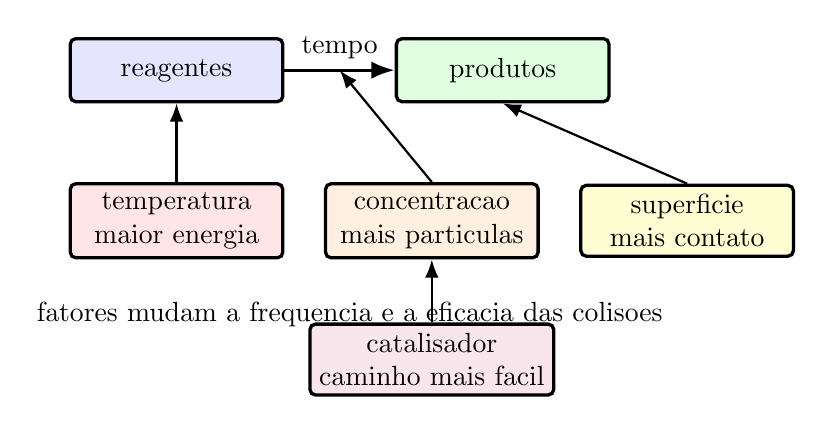
\begin{tikzpicture}[>=Latex,node distance=0.9cm]
  \tikzstyle{box}=[draw,rounded corners=2pt,very thick,minimum width=2.7cm,minimum height=0.8cm,align=center]
  \node[box,fill=blue!10] (reag) {reagentes};
  \node[box,fill=green!12,right=1.4cm of reag] (prod) {produtos};
  \draw[very thick,->] (reag) -- (prod) node[midway,above] {tempo};
  \node[box,fill=red!10,below=1.0cm of reag] (temp) {temperatura\\maior energia};
  \node[box,fill=orange!12,right=0.5cm of temp] (conc) {concentracao\\mais particulas};
  \node[box,fill=yellow!18,right=0.5cm of conc] (sup) {superficie\\mais contato};
  \node[box,fill=purple!10,below=0.8cm of conc] (cat) {catalisador\\caminho mais facil};
  \draw[thick,->] (temp.north) -- (reag.south);
  \draw[thick,->] (conc.north) -- ($(reag)!0.5!(prod)$);
  \draw[thick,->] (sup.north) -- (prod.south);
  \draw[thick,->] (cat.north) -- (conc.south);
  \node[align=center] at (2.2,-3.1) {fatores mudam a frequencia e a eficacia das colisoes};
\end{tikzpicture}
\end{document}
